\documentclass[a4paper]{article}
\usepackage{tikz}
\usetikzlibrary{petri,arrows}
\usepackage{amstext}

\begin{document}


%% TikZ style options %%
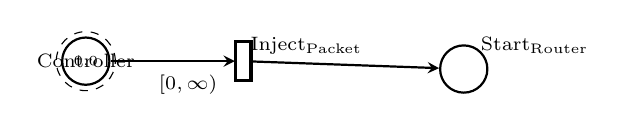
\begin{tikzpicture}[font=\scriptsize, xscale=1, yscale=1]
%% the figure can be scaled by changing xscale and yscale
%% positions of place/transition labels that are currently fixed to label=135 degrees
%% can be adjusted so that they do not cover arcs
%% similarly the curving of arcs can be done by adjusting bend left/right=XX
%% labels may be slightly skewed compared to the tapaal drawing due to rounding.
%% This can be adjusted by tuning the coordinates of the label
\tikzstyle{arc}=[->,>=stealth,thick]
\tikzstyle{transportArc}=[->,>=diamond,thick]
\tikzstyle{inhibArc}=[->,>=o,thick]
\tikzstyle{every place}=[minimum size=6mm,thick]
\tikzstyle{every transition} = [fill=black,minimum width=2mm,minimum height=5mm]
\tikzstyle{every token}=[fill=white,text=black]
\tikzstyle{sharedplace}=[place,minimum size=7.5mm,dashed,thin]
\tikzstyle{sharedtransition}=[transition, fill opacity=0, minimum width=3.5mm, minimum height=6.5mm,dashed]
\tikzstyle{urgenttransition}=[place,fill=white,minimum size=2.0mm,thin]\tikzstyle{uncontrollabletransition}=[transition,fill=white,draw=black,very thick]
%% TikZ-figure elements %%
\node[place, structured tokens={0.0},] at (2.0,-2.7) (Controller) {};
\node[sharedplace] at (Controller.center) { };
%% label for place Controller
\draw (2.0,-2.7) node[align=left] {$\mathrm{Controller}$};
\node[place] at (6.8,-2.8) (Start_Router) {};
%% label for place Start_Router
\draw (7.7,-2.5) node[align=left] {$\mathrm{Start_{Router}}$};
\node[transition] at (4.0,-2.7) (Inject_Packet) {};
\node[uncontrollabletransition] at (Inject_Packet.center) { };
%% label for transition Inject_Packet
\draw (4.8,-2.5) node  {$\mathrm{Inject_{Packet}}$};
\draw[arc] (Controller) to[bend right=0] (Inject_Packet) {};
%% Label for arc between Controller and Inject_Packet
\draw (3.3,-3.0) node {$\mathrm{[0,\infty)}$};
\draw[arc] (Inject_Packet) to[bend right=0] (Start_Router) {};
\end{tikzpicture}
\end{document}
